\chapter{Evolution of the simulator}
	\section{Basic 2 car setup with IDM}\label{sec:base2car}
		Equation \ref{eq:numerical_idm} can be solved with an Explicit Euler. To test the model a basic setup was implemented in \textsc{Matlab}. The visual representation of the setup can be seen on figure \ref{fig:basic2car}.
		\begin{figure}[ht]
			\centering
			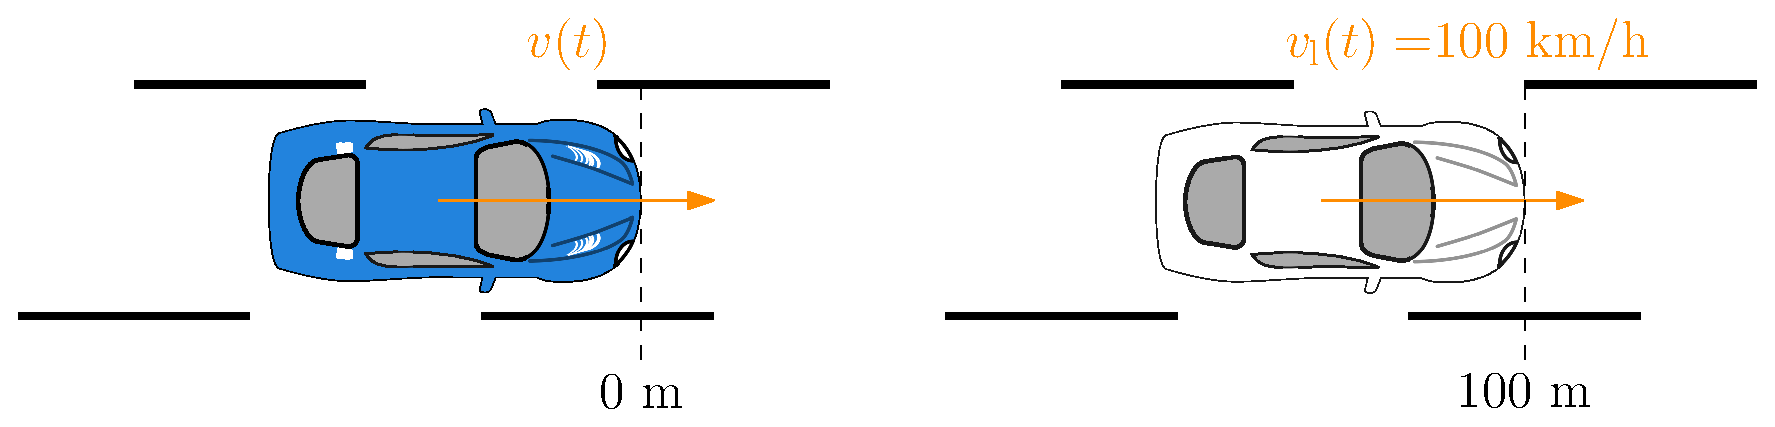
\includegraphics[width=.95\textwidth]{common/basic_2_car}
			\caption{Basic setup with 2 cars}
			\label{fig:basic2car}
		\end{figure}
		The leading car has a constant 100 km/h velocity. The following car - which is modeled with IDM - has an initial velocity of 100 km/h as well. The second car is 100 meters behind the other car. The parameters of following car can be seen in Table \ref{tab:idm_params}. The parameters have been chosen based on literature from [TODO:reference here].
		\begin{table}[ht]
			\begin{center}
				\begin{tabular}{ |c|c|c| }
					\hline
					$a_{\rm max}$ & $1.5$ & $\rm m/s^2$ \\
					$b_{\rm max}$ & $1.67$ & $\rm m/s^2$ \\
					$v_{\rm d}$ & $130$ & km/h \\
					$T$ & $1.8$ & s \\
					$h_0$ & $2$ & m \\
					$\rm \delta$ & $4$ & - \\
					$L$ & $4.5$ & m \\
					\hline
				\end{tabular}
			\end{center}
			\caption{Intelligent Driver Model parameters}
			\label{tab:idm_params}
		\end{table}
		The simulation was run until 100 seconds. Figure \ref{fig:basic2car_case_1} shows the result. The initial gap between the cars is greater than the second car's desired headway, consequently the vehicle will accelerate. The gap between the vehicles starts to decrease. At a certain time (around $t =$ 10) the second car starts to decelerate slowly based on the velocity difference and the decreasing headway. It will reach the desired safe gap at some point and will have exactly the same speed as the car before. It will maintain its desired headway.
		\begin{figure}[ht]
			\centering
			\begin{minipage}{.5\textwidth}
				\centering
				\includegraphics{ee/basic_2_car_headaway_case_1_2}
			\end{minipage}\hfill
			\begin{minipage}{.5\textwidth}
				\centering
				\includegraphics{ee/basic_2_car_velocity_case_1_2}
			\end{minipage}
			\caption{Following car's headway and velocity in Setup 1}
			\label{fig:basic2car_case_1}
		\end{figure}

		Another simulation was run with the same configuration except that the first car's front is set to be at 40 meters instead of 100. Figure \ref{fig:basic2car_case_2} shows the result. In this case the gap between cars is less than the second vehicle's desired safety headway. So it will decelerate first than accelerate to reach the desired gap. Fundamentally the same happened but in the opposite direction.
		\begin{figure}[ht]
			\centering
			\begin{minipage}{.5\textwidth}
				\centering
				\includegraphics{ee/basic_2_car_headaway_case_2_2}
			\end{minipage}\hfill
			\begin{minipage}{.5\textwidth}
				\centering
				\includegraphics{ee/basic_2_car_velocity_case_2_2}
			\end{minipage}
			\caption{Following car's headway and velocity in Setup 2}
			\label{fig:basic2car_case_2}
		\end{figure}
		Both examples showed that the stationary state does not depend on the initial gap. After a little bit of time the second car has reached the desired safety gap (which is around 64.5 meters) and the 100 km/h speed in both cases.
	\section{Model behavior verification}
		In Section \ref{sec:base2car} two examples were shown where the model produced the same stationary state for different initial conditions. Stationary state means that the vehicle's acceleration is zero. So equation \ref{eq:aidm} modifies as followings in a stationary state:
		\begin{equation}
		1 - \left ( \frac{v_{\rm stac}}{v_{\rm d}} \right )^{\rm \delta} - \left ( \frac{h_0+v_{\rm stac}\cdot T+\frac{v_{\rm stac}(v_{\rm stac}-v_{\rm lead,stac})}{2\sqrt{\amax \bmax}}}{x_{\rm lead,0}+v_{\rm lead, stac}\cdot t - L_{\rm lead} - (x_{0} + v_{\rm stac}\cdot t)} \right )^2=0\,,
		\label{eq:aidm_stac1}
		\end{equation}
		There is an other consequence of this situation as well. As it can be seen in the examples, cars' velocities were equal, which means:
		\begin{equation}
			v_{\rm stac}=v_{\rm lead,stac}\,,
		\end{equation}
		so Equation \ref{eq:aidm_stac1} further simplifies to:
		\begin{equation}
			1 - \left ( \frac{v_{\rm stac}}{v_{\rm d}} \right )^{\rm \delta} - \left ( \frac{h_0+v_{\rm stac}\cdot T}{x_{\rm lead,0}-x_{0} - L_{\rm lead}} \right )^2=0\,.
			\label{eq:aidm_stac2}
		\end{equation}
		It can be stated that the stationary gap between the vehicles equals to the denominator of the second fraction expression:
		\begin{equation}
		x_{\rm lead,0}-x_{0} - L_{\rm lead}=h_{\rm stac}\,.
		\label{eq:aidm_stac3}
		\end{equation}
		Expressions \ref{eq:aidm_stac2} and \ref{eq:aidm_stac3} show that $v_{\rm stac}$ only depends on $h_{\rm stac}$. Everything else in the equations is a parameter of the model or initial condition. Consequently every stationary gap has a corresponding speed value. Using \textsc{Matlab} fsolve method Equation \ref{eq:aidm_stac2} can be solved. Plot of the result can be seen on Figure \ref{fig:aidm_stac}.
		\begin{figure}[ht]
			\centering
			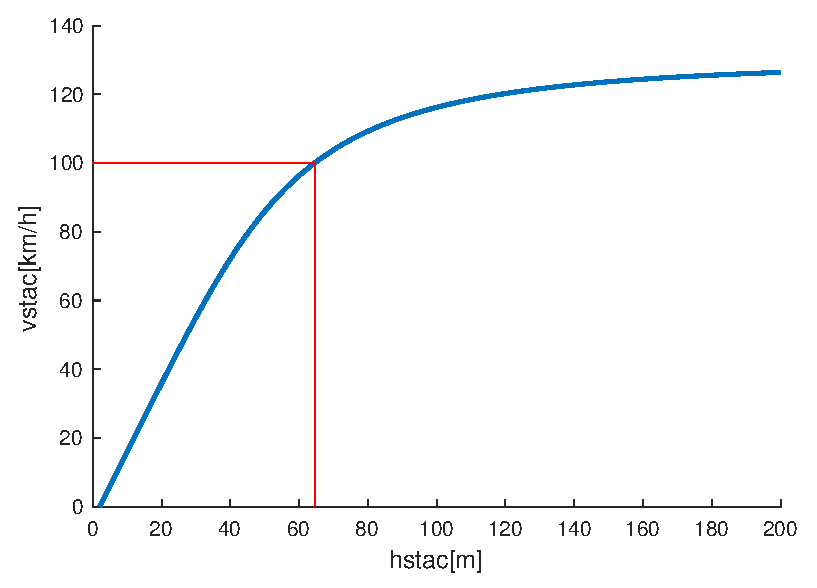
\includegraphics{check/check_stationary_states}
			\caption{Stationary velocity based on stationary headway}
			\label{fig:aidm_stac}
		\end{figure}

		In the examples of Section \ref{sec:base2car} the stationary gap between the vehicles was around 64.5 meters and the velocity was 100 km/h. Figure \ref{fig:aidm_stac} shows exactly the same values. It can be stated that the model and the numerical solver is working as expected. Note that the bumper to bumper or traffic jam distance ($h_0$) appears on the horizontal axis and it has a zero velocity value.
	\section{Solver verification}
		A custom Explicit Euler solver was implemented to solve equation \ref{eq:numerical_idm} numerically. However \textsc{Matlab} provides built-in solvers for differential equation systems like IDM. It has a solver called ode45. It is a 4th order numerical solver which is capable of changing some of its parameters (e.g.: time step) based on the system's behavior. So theoretically it is a better choice over a custom implemented Explicit Euler to solve differential equation systems. It also provides a verification to the custom implemented solver. 
		\begin{figure}[ht]
			\centering
			\begin{minipage}{.5\textwidth}
				\centering
				\includegraphics{ode/basic_2_car_headaway_case_1_2}
			\end{minipage}\hfill
			\begin{minipage}{.5\textwidth}
				\centering
				\includegraphics{ode/basic_2_car_velocity_case_1_2}
			\end{minipage}
			\caption{Following car's headway and velocity in Setup 1 with ode45}
			\label{fig:basic2car_case_1_ode}
		\end{figure}
		\begin{figure}[ht]
			\centering
			\begin{minipage}{.5\textwidth}
				\centering
				\includegraphics{ode/basic_2_car_headaway_case_2_2}
			\end{minipage}\hfill
			\begin{minipage}{.5\textwidth}
				\centering
				\includegraphics{ode/basic_2_car_velocity_case_2_2}
			\end{minipage}
			\caption{Following car's headway and velocity in Setup 2  with ode45}
			\label{fig:basic2car_case_2_ode}
		\end{figure}

		The same two examples were implemented with ode45 as before in Section \ref{sec:base2car} with EE.
		It can be seen on Figure \ref{fig:basic2car_case_1_ode} and \ref{fig:basic2car_case_2_ode} that the solutions are exactly the same as before, consequently the custom made solver is working as expected.
	\section{Solution for n cars}
		The simulator works as expected for 2 cars simulations. It is time to implement an n-car simulation as well. The simulator still uses the built-in ode45 function to solve the differential equation system so the only task is to produce $\dot{y}$. However the dimension of the system grows from 4 to 2n. The visual representation of the setup can be seen on Figure \ref{fig:basic_n_car}. The first car will have a constant velocity of 100 km/h so $\dot{y}_1 = 100$ and $\dot{y}_2 = 0$, since there is no acceleration.
		\begin{figure}[ht]
			\centering
			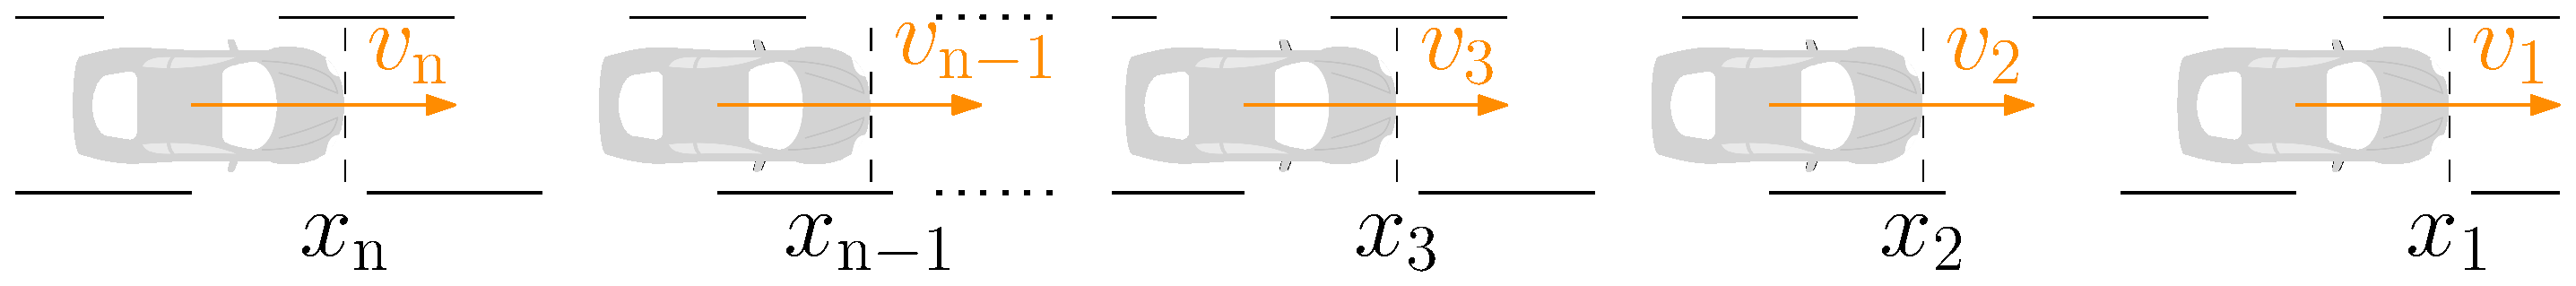
\includegraphics[width=\textwidth]{common/basic_n_car}
			\caption{n-car setup}
			\label{fig:basic_n_car}
		\end{figure}
		Unfortunately the previously used implementation is not good enough to produce $\dot{y}$. The problem is  that to be able to calculate vehicle n's position and velocity the solver needs to have vehicle n-1's position and velocity. To make it easy to read let us introduce function $f$ which represents equation \ref{eq:numerical_idm}. Than $\dot{y}$ looks like the following:
		\begin{equation}
			\dot{y}=
			\begin{pmatrix}
				100\\
				0\\
				f_1(v_{2})\\
				f_2(v_{2}, x_{2},v_{1}, x_{1})\\
				f_1(v_{3})\\
				f_2(v_{3}, x_{3},v_{2}, x_{2})\\
				\vdots\\
				f_1(v_{\rm n-1})\\
				f_2(v_{n-1}, x_{n-1},v_{n-2}, x_{n-2})\\
				f_1(v_{\rm n})\\
				f_2(v_{n}, x_{n},v_{n-1}, x_{n-1})
			\end{pmatrix}\,.
			\label{eq:n_ode_math}
		\end{equation}
		A couple of setups were made with n=5 to test the new n-car solver. The vehicles' IDM parameters were unchanged, it can be found in Table \ref{tab:idm_params}.
		\subsection*{Case 1}
		The initial positions and velocities of the cars can be seen on Table \ref{tab:node_case1}.
		\begin{table}
			\centering
			\begin{tabular}{ |c|c|c| }
				\hline
				n [-] & $x$ [m] & $v$ [km/h]\\
				\hline
				1 & 400 & 100 \\
				2 & 300 & 100 \\
				3 & 200 & 100 \\
				4 & 100 & 100 \\
				5 & 0 & 100 \\
				\hline
			\end{tabular}
			\caption{Case 1}
			\label{tab:node_case1}
		\end{table}
		The result of the simulation is on Figure \ref{fig:node_case1}. Every car's leader is a bit further than their desired safety headway so every car is accelerating then they try to maintain their desired headway. The same phenomenon can be seen in the 2-car simulation as expected.
		\begin{figure}
			\centering
			\begin{minipage}{.5\textwidth}
				\centering
				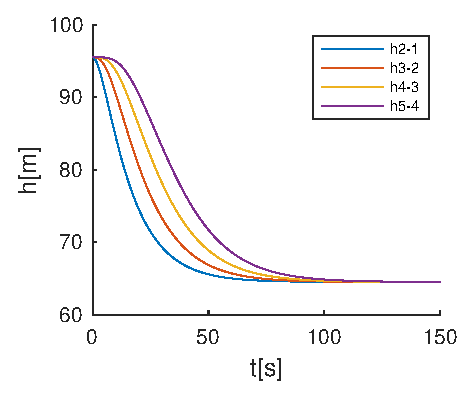
\includegraphics{node/n_car_headway_case1}
			\end{minipage}\hfill
			\begin{minipage}{.5\textwidth}
				\centering
				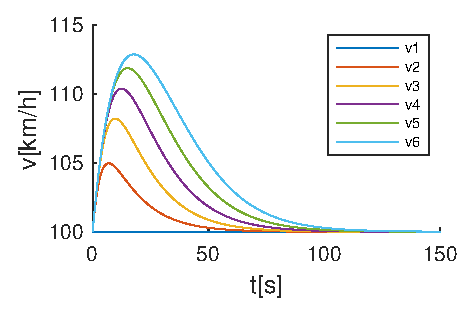
\includegraphics{node/n_car_velocity_case1}
			\end{minipage}
			\caption{Case 1}
			\label{fig:node_case1}
		\end{figure}
		\subsection*{Case 2}
		The initial positions and velocities of the cars can be seen on Table \ref{tab:node_case2}.
		\begin{table}
			\centering
			\begin{tabular}{ |c|c|c| }
				\hline
				n [-] & $x$ [m] & $v$ [km/h]\\
				\hline
				1 & 160 & 100 \\
				2 & 120 & 100 \\
				3 & 80 & 100 \\
				4 & 40 & 100 \\
				5 & 0 & 100 \\
				\hline
			\end{tabular}
			\caption{Case 2}
			\label{tab:node_case2}
		\end{table}
		The result of the simulation is on Figure \ref{fig:node_case2}. Every car's leader is a bit closer than their desired safety headway so every car is decelerating then they try to maintain their desired headway. The same phenomenon can be seen in the 2-car simulation as well.
		\begin{figure}
			\centering
			\begin{minipage}{.5\textwidth}
				\centering
				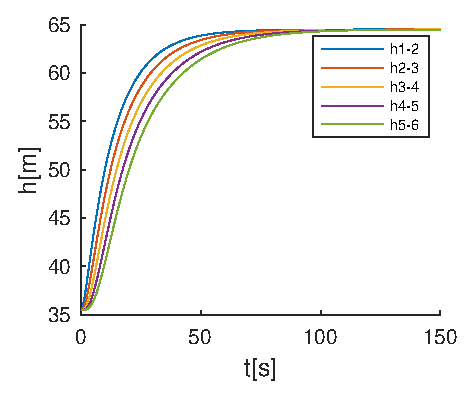
\includegraphics{node/n_car_headway_case2}
			\end{minipage}\hfill
			\begin{minipage}{.5\textwidth}
				\centering
				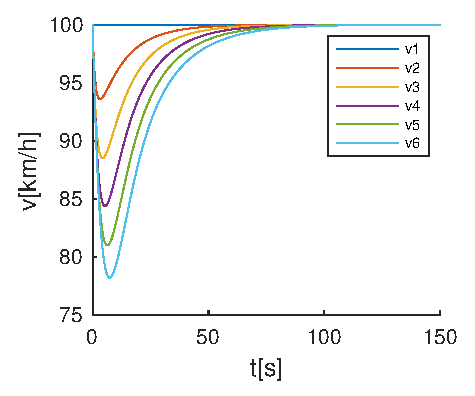
\includegraphics{node/n_car_velocity_case2}
			\end{minipage}
			\caption{Case 2}
			\label{fig:node_case2}
		\end{figure}
		\subsection*{Case 3}
		The initial positions and velocities of the cars can be seen on Table \ref{tab:node_case3}.
		\begin{table}
			\centering
			\begin{tabular}{ |c|c|c| }
				\hline
				n [-] & $x$ [m] & $v$ [km/h]\\
				\hline
				1 &  280 & 100 \\
				2 & 180 & 100 \\
				3 & 140 & 100 \\
				4 & 40 & 100 \\
				5 & 0 & 100 \\
				\hline
			\end{tabular}
			\caption{Case 3}
			\label{tab:node_case3}
		\end{table}
		The result of the simulation is on Figure \ref{fig:node_case3}. In case 3 some of the cars are closer to their leader than their desired safety gap and there are cars which have more headway than their safety gap. As a result the former ones will decelerate, the latter ones will accelerate to reach the desired headway.
		\begin{figure}
			\centering
			\begin{minipage}{.5\textwidth}
				\centering
				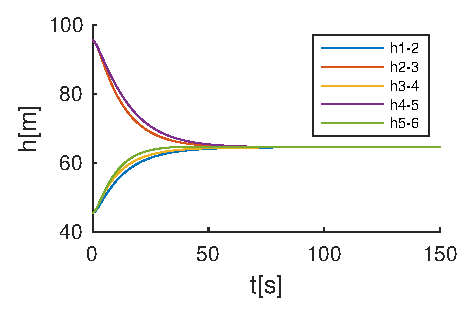
\includegraphics{node/n_car_headway_case3}
			\end{minipage}\hfill
			\begin{minipage}{.5\textwidth}
				\centering
				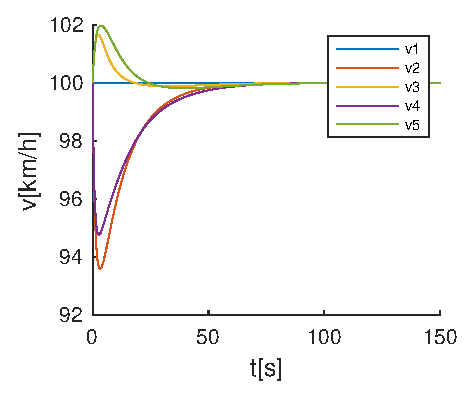
\includegraphics{node/n_car_velocity_case3}
			\end{minipage}
			\caption{Case 3}
			\label{fig:node_case3}
		\end{figure}
		\subsection*{Case 4}
		The initial positions and velocities of the cars can be seen on Table \ref{tab:node_case4}.
		\begin{table}
			\centering
			\begin{tabular}{ |c|c|c| }
				\hline
				n [-] & $x$ [m] & $v$ [km/h]\\
				\hline
				1 &  280 & 100 \\
				2 & 180 & 80 \\
				3 & 140 & 120 \\
				4 & 40 & 115 \\
				5 & 0 & 70 \\
				\hline
			\end{tabular}
			\caption{Case 4}
			\label{tab:node_case4}
		\end{table}
		The result of the simulation is on Figure \ref{fig:node_case4}.
		\begin{figure}
			\centering
			\begin{minipage}{.5\textwidth}
				\centering
				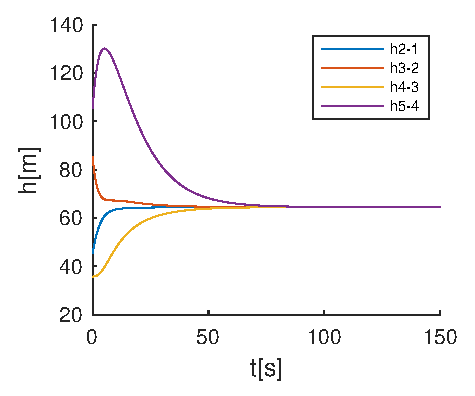
\includegraphics{node/n_car_headway_case4}
			\end{minipage}\hfill
			\begin{minipage}{.5\textwidth}
				\centering
				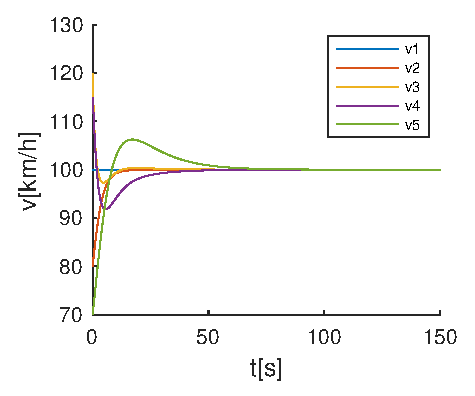
\includegraphics{node/n_car_velocity_case4}
			\end{minipage}
			\caption{Case 4}
			\label{fig:node_case4}
		\end{figure}
